\documentclass[../../thesis.tex]{subfiles}
\graphicspath{{\subfix{../../resources/}}}
\begin{document}
\section{Preliminary tests}
In order to answer our research question, we first need to determine an effective
setup for the group sampling algorithm. For this, we try to answer two questions
in this section.


\begingroup
\renewcommand{\arraystretch}{1.5}
\begin{flushleft}
    \begin{tabular}{lp{0.9\textwidth}}
        $Q_{1}$ & Which variant of group sampling is more effective?                                        \\
                & In \autoref{sec:group_sampling:creation_of_groups}, two variants to create groupings with
        the help of an SAT-Solver are described. While the creation of the influence model is the same,
        the actual result is dependent on the groupings created. To determine the superior strategy
        to create groupings, both variants are tested on our real-world examples.                           \\
        $Q_{2}$ & How can we determine the group size?                                                      \\
                & The results of the group sampling algorithm are dependent on the group size used during
        sampling. With bigger groups, more information for a single feature can be extracted, but it comes at the
        cost of more actual measurements required. We try to find a group size, which minimizes
        the measurements required while still giving us a decent model. As with $Q_1$, this is done by testing
        the group sampling on our real-world datasets with different group sizes.
    \end{tabular}
\end{flushleft}
\endgroup

To answer those question, we sample our four real-world examples with both variants described
in \autoref{sec:group_sampling:creation_of_groups} and train an influence model as described in
\autoref{sec:optimization:stepwise_influence}.
This is done with 2,3,4 and 5 groups and a sample size of one to 20.
The models are evaluated on a test dataset of 100 samples and the MAPE value for each is calculated.
The results can be found in \autoref{fig:graph:grouping_method_and_size_real}.
Worth mentioning here is, that the sample size reflects the actual number of measurements needed, not the
number of groupings done.

\subsubsection{$Q_1$ Which variant of group sampling is more effective?}
When comparing the models created by the first and second variants, "Hamming-Distance" and "Independent Feature",
a fundamental flaw in the first variant is visible. If we look at the Apache dataset, for the group sizes of
3,4 and 5, the model has a constant MAPE value, indicating that the model does not learn the characteristics of the system.
This is caused by the fact, that the number of features for each group, which the SAT-Solver tries to enable is smaller
than the number of required features. If we look at \autoref{eq:group_sampling:creation_of_groups:hamming:no_of_features}
the number of features per group is 8, 6, 4 for the group sizes of 3, 4, 5 respectively on the Apache dataset.
With 10 required features on the Apache dataset, the SAT-Solver can not create a group with less than the required
amount of features. This results in groups, where only the required features are enabled and thus completely
leaving out all other features in the dataset.

Even if the inadequate group sizes are ignored, the grouping variant based on maximizing the Hamming distance
is producing worse results than the grouping of independent features.


\subsubsection{$Q_2$ How can we determine the group size?}

The group sizes play a role in the determination of influential parameters.
With too many features in a group, influential parameters are grouped together more often,
making it harder to determine their influence. With too few features in a group, more
measurements need to be made, which defeats the purpose of group sampling and starts to resemble an OAT-approach.

We have already seen that the grouping method based on the hamming distance does not work properly for
certain group sizes. This method severely limits the selectable group sizes and makes it even harder
to pick an appropriate group size. While selecting a meaningful group size with this method is possible if
the amount of mutually exclusive groups and independent features is known, we will focus on the method
of grouping independent features, since this method proves to be superior.

With the method of grouping independent features, the group size does not affect the amount of mutually exclusive features
in a group. The group size only specifies how many independent features are in a group.
This, for example, explains why in the Apache dataset the resulting
accuracy of the model is not significantly changing. The influential feature in this dataset \textit{keepalive} is part of a mutually exclusive group.
We also can see, especially with only a few independent features, the group size plays close to no role
in the accuracy of the model. Whereas the overall sample size plays a more significant role.
On larger datasets with more independent features, the group size plays a more significant role.
With more groups and fewer features in one group, the model gets more accurate. 
We can see this in \autoref{fig:graph:grouping_method_and_size_syn}. 
The major drawback with more groups is the increased amount of measurements that have to be 
taken to determine the influence for each group. During our tests, we noticed diminishing returns 
with fewer features in a group until each group consists of a minimal amount of features.
Group sizes of around one-tenth of the number of independent features but no less than 2 resulted, on average,
in the most accurate model.



\begin{figure}[!htp]
    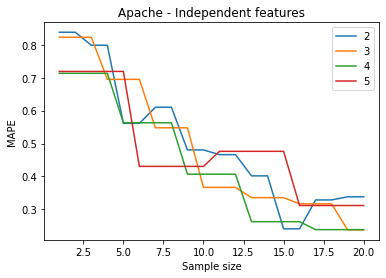
\includegraphics[width=0.5\textwidth]{graphs/apache_group_sizes.png}
    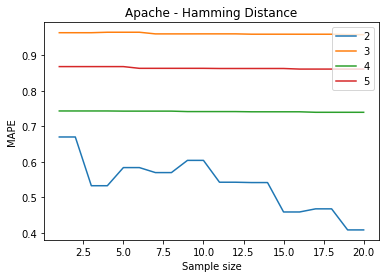
\includegraphics[width=0.5\textwidth]{graphs/apache_group_sizes_hamming.png}
    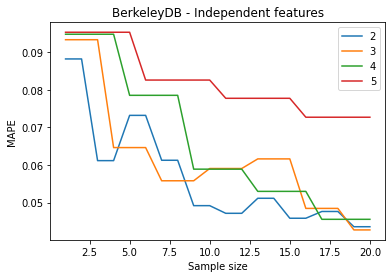
\includegraphics[width=0.5\textwidth]{graphs/berkley_group_sizes.png}
    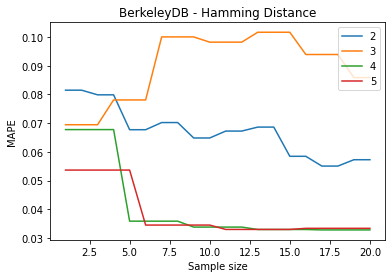
\includegraphics[width=0.5\textwidth]{graphs/berkley_group_sizes_hamming.png}
    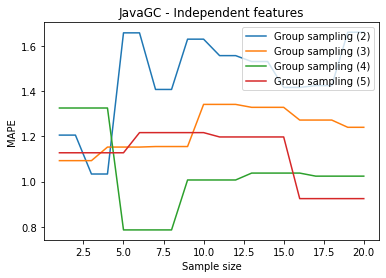
\includegraphics[width=0.5\textwidth]{graphs/javagc_group_sizes.png}
    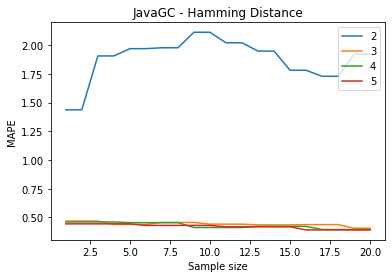
\includegraphics[width=0.5\textwidth]{graphs/javagc_group_sizes_hamming.png}
    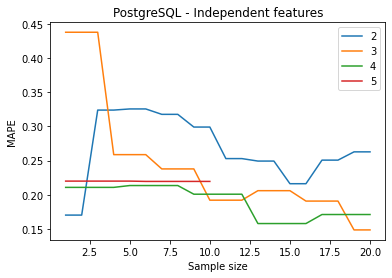
\includegraphics[width=0.5\textwidth]{graphs/postgre_group_sizes.png}
    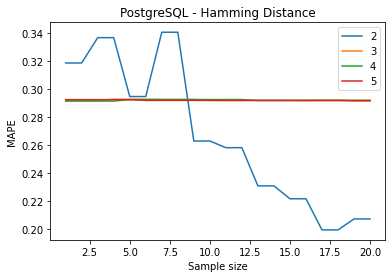
\includegraphics[width=0.5\textwidth]{graphs/postgre_group_sizes_hamming.png}
    \caption[Different group sizes on the real world datasets]{
        Different group sizes on the real world datasets.
    }\label{fig:graph:grouping_method_and_size_real}
\end{figure}

\begin{figure}[!htp]
    \begin{center}
        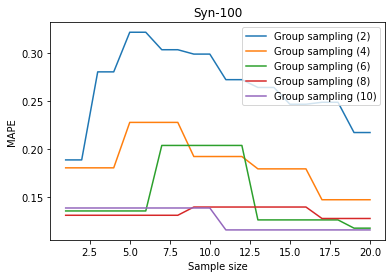
\includegraphics[width=0.5\textwidth]{graphs/syn-100_group_sizes.png}
    \end{center}
    \caption[Different group sizes on the SYN-100 datasets]{
        Different group sizes on the SYN-100 datasets.
    }\label{fig:graph:grouping_method_and_size_syn}
\end{figure}



\end{document}